\documentclass[tikz,border=10pt]{standalone}
\usepackage{tikz}
\usetikzlibrary{shapes,arrows,positioning,shadows,fit}

\begin{document}

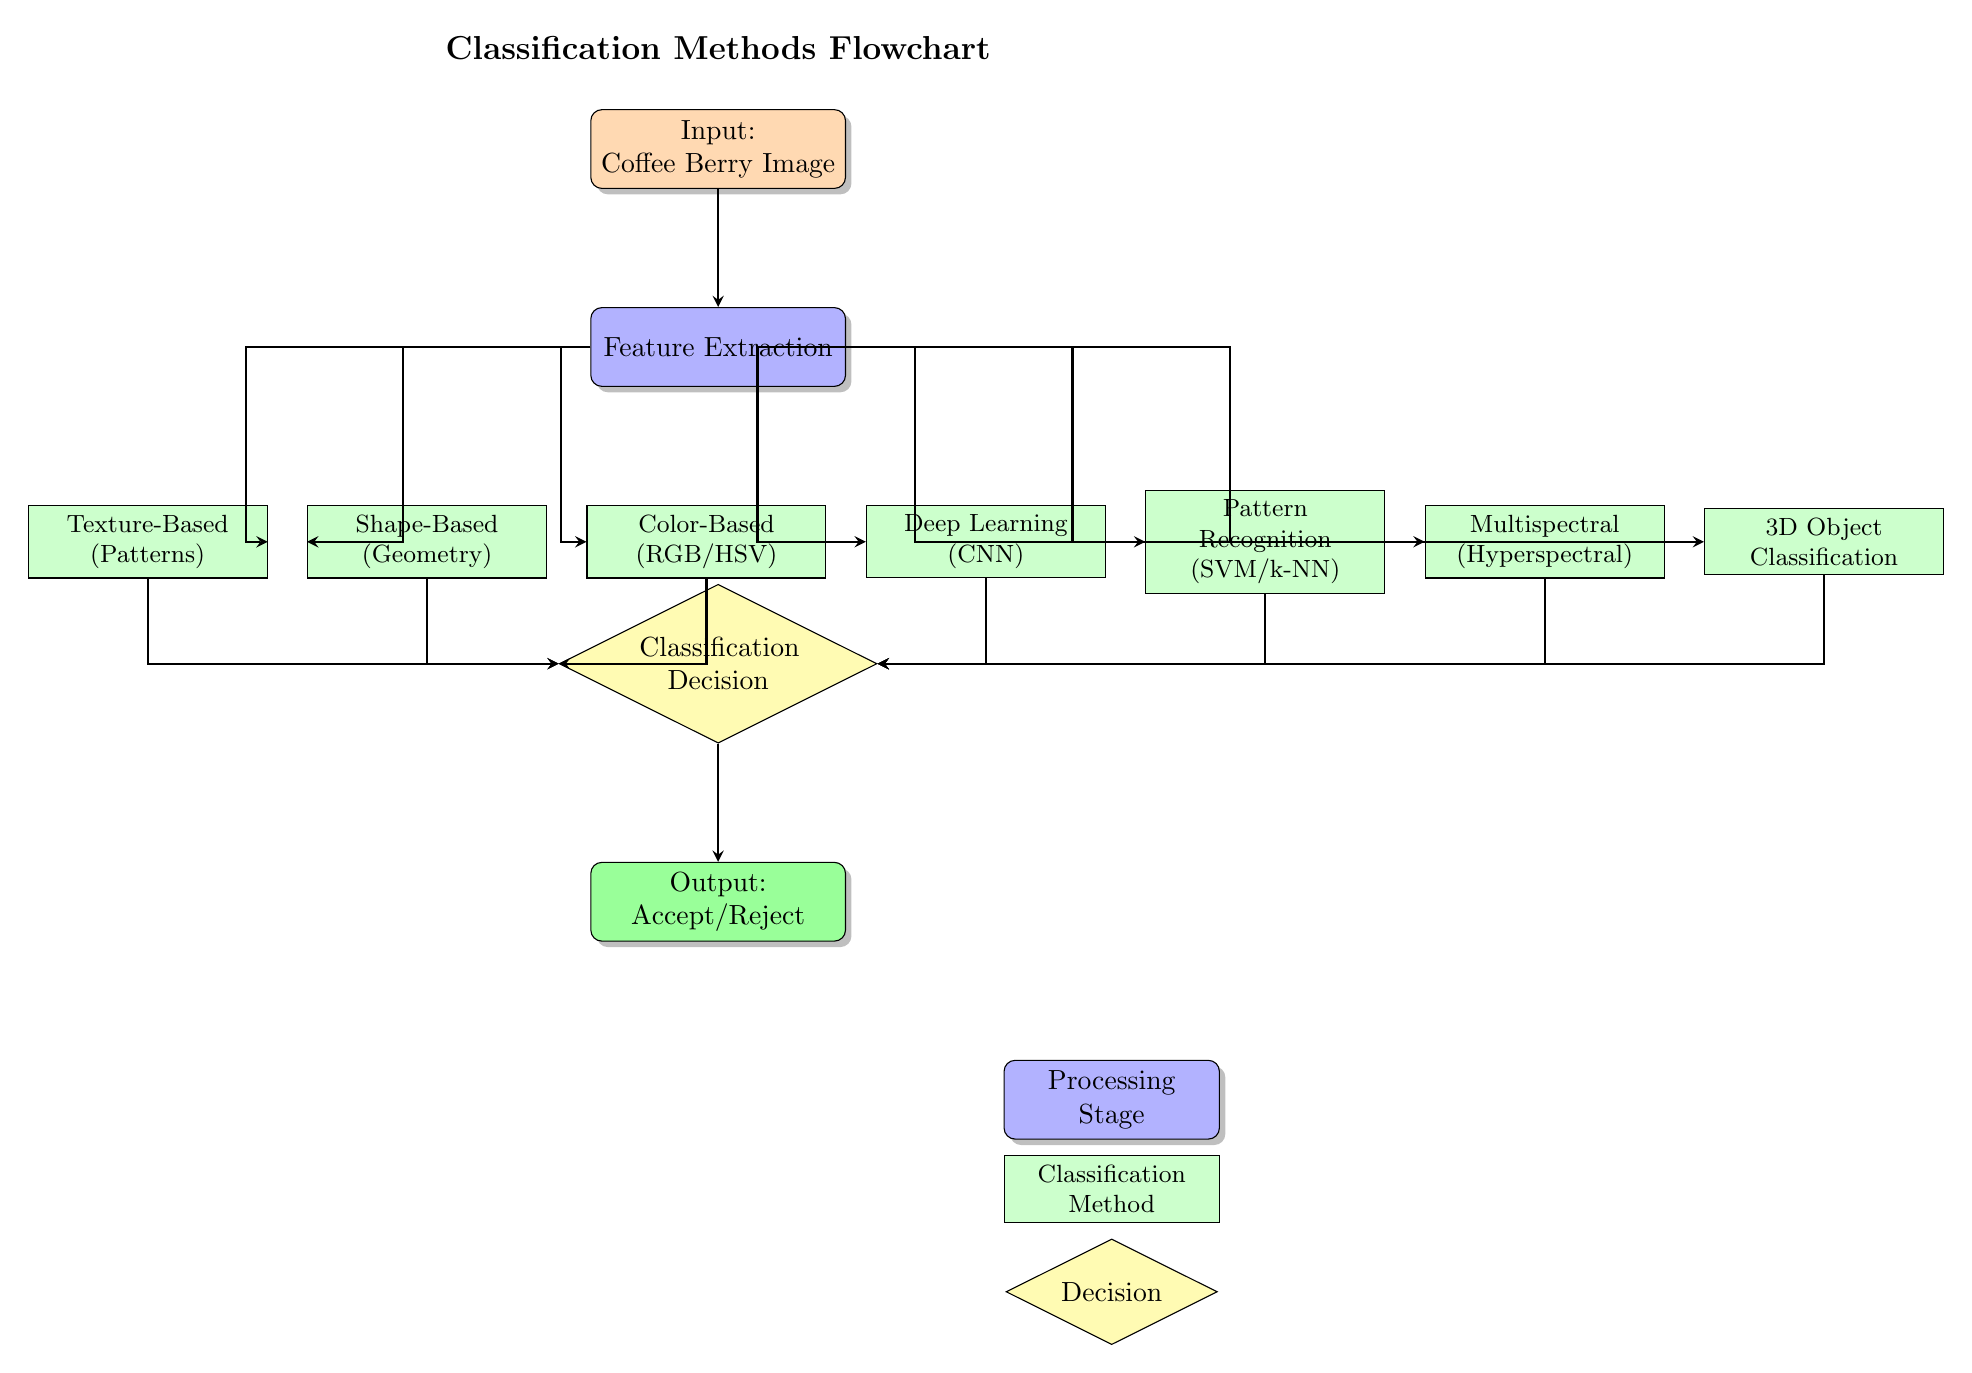
\begin{tikzpicture}[
    node distance=1.5cm,
    process/.style={rectangle, draw, fill=blue!30, text width=3cm, text centered, rounded corners, minimum height=1cm, drop shadow},
    method/.style={rectangle, draw, fill=green!20, text width=2.8cm, text centered, minimum height=0.8cm, font=\small},
    decision/.style={diamond, draw, fill=yellow!30, text width=2cm, text centered, minimum height=1cm, aspect=2},
    arrow/.style={thick,->,>=stealth}
]

% Start
\node[process, fill=orange!30] (start) {Input:\\Coffee Berry Image};

% Main classification branches
\node[process, below=of start] (features) {Feature Extraction};

% Seven classification methods
\node[method, below left=1.5cm and -3cm of features] (color) {Color-Based\\(RGB/HSV)};
\node[method, left=0.5cm of color] (shape) {Shape-Based\\(Geometry)};
\node[method, left=0.5cm of shape] (texture) {Texture-Based\\(Patterns)};
\node[method, right=0.5cm of color] (dl) {Deep Learning\\(CNN)};
\node[method, right=0.5cm of dl] (pattern) {Pattern\\Recognition\\(SVM/k-NN)};
\node[method, right=0.5cm of pattern] (multi) {Multispectral\\(Hyperspectral)};
\node[method, right=0.5cm of multi] (3d) {3D Object\\Classification};

% Decision node
\node[decision, below=2.5cm of features] (classify) {Classification\\Decision};

% Output
\node[process, below=of classify, fill=green!40] (output) {Output:\\Accept/Reject};

% Arrows from start
\draw[arrow] (start) -- (features);
\draw[arrow] (features) -- ++(-6,0) |- (texture);
\draw[arrow] (features) -- ++(-4,0) |- (shape);
\draw[arrow] (features) -- ++(-2,0) |- (color);
\draw[arrow] (features) -- ++(0.5,0) |- (dl);
\draw[arrow] (features) -- ++(2.5,0) |- (pattern);
\draw[arrow] (features) -- ++(4.5,0) |- (multi);
\draw[arrow] (features) -- ++(6.5,0) |- (3d);

% Arrows to classification
\draw[arrow] (texture) |- (classify);
\draw[arrow] (shape) |- (classify);
\draw[arrow] (color) |- (classify);
\draw[arrow] (dl) |- (classify);
\draw[arrow] (pattern) |- (classify);
\draw[arrow] (multi) |- (classify);
\draw[arrow] (3d) |- (classify);

% Arrow to output
\draw[arrow] (classify) -- (output);

% Title
\node[above=0.5cm of start, font=\bfseries\large] (title) {Classification Methods Flowchart};

% Legend boxes
\node[process, below right=1.5cm and 2cm of output, text width=2.5cm, fill=blue!30] (leg1) {Processing Stage};
\node[method, below=0.2cm of leg1, text width=2.5cm] (leg2) {Classification Method};
\node[decision, below=0.2cm of leg2, text width=1.5cm] (leg3) {Decision};

\end{tikzpicture}

\end{document}
